\documentclass[10pt, a4paper,spanish]{article}

\usepackage[utf8]{inputenc}
\usepackage[spanish]{babel}

\usepackage[T1]{fontenc}

\usepackage[hmarginratio=1:1,top=32mm,columnsep=20pt]{geometry}
\usepackage[hang, small,labelfont=bf,up,textfont=it,up]{caption}

\usepackage{float}

\usepackage{amsmath}

\usepackage{listings}

\usepackage{enumitem}

\usepackage{hyperref}

\usepackage{graphicx}



\usepackage{titlesec}
\renewcommand\thesection{\Roman{section}}
\renewcommand\thesubsection{\Roman{subsection}}
\titleformat{\section}[block]{\large\scshape\centering}{\thesection.}{1em}{}
\titleformat{\subsection}[block]{\large}{\thesubsection.}{1em}{}

\usepackage{fancyhdr}
\pagestyle{fancy}
\fancyhead{}
\fancyfoot{}
\fancyhead[C]{ \today \ $\bullet$ Grámaticas y Lenguajes Formales $\bullet$ Práctica 1}
\fancyfoot[RO]{\thepage}

%-------------------------------------------------------------------------------
%	Seccion titulo
%-------------------------------------------------------------------------------

\title{\vspace{-15mm}\fontsize{24pt}{10pt}\selectfont\textbf{Procesamiento de ficheros CSV}}

\author{
	Iván López de Munain Quintana
}

\date{\today}



%-------------------------------------------------------------------------------
\begin{document}

	\maketitle % Insert title

	\thispagestyle{fancy} % All pages have headers and footers


%-------------------------------------------------------------------------------
%	TEXT
%-------------------------------------------------------------------------------



\textbf{\section{Introducción.\\\\}}

\paragraph{}
\noindent En esta primera entrega se va a poner en práctica los conocimientos adquiridos de los comandos \textit{awk}, \textit{sed} y \textit{egrep} para el procesamiento de ficheros CSV. En suma, se van a mostrar cómo escribir programas \textit{bash} y cómo hacer que los ficheros sean ejecutables, entre otras cosas. Antes de comenzar con los ejercicios de la práctica tenemos que descargar los datos que se encuentran en \small{\url{https://datosabiertos.jcyl.es/web/jcyl/risp/es/ciencia-tecnologia/
general/1284166186527.csv}} . Para conseguir esto se han ejecutado los siguientes comandos (cabe recordar que se han escrito en el fichero \textit{guion} que se ha convertido en ejecutable mediante la orden \textit{chmod $+$x guion}):
\begin{lstlisting}

    #Comandos incluidos en guion 
    #crear el directorio para almacenar los datos
    mkdir data  
    
    #descarga del conjunto de datos y almacenamiento en CataDatosRaw.csv
    curl https://datosabiertos.jcyl.es/web/jcyl/risp/es/ciencia-tecnologia/
    general/1284166186527.csv > data/CataDatosRaw.csv 
    
\end{lstlisting}

\noindent \\ Posteriormente se nos pide que cambiemos la codificación del juego de caracteres del fichero \textit{CataDatosRaw.csv} de la forma ISO-8859-1 a UTF-8 y almacenemos el resultado en \textit{data/CataDatosJCyL.csv} mediante la siguiente orden: 

\begin{lstlisting}

    #Comando incluido en guion 
    iconv -f ISO-8859-1 -t UTF-8 data/CataDatosRaw.csv > data/CataDatosJCyL.csv
    
\end{lstlisting}

\noindent \\ Una vez realizada toda la preparación de los datos ya estamos preparados para normalizar el fichero CSV \textit{CataDatosJCyL.csv} como se mostrará en el siguiente apartado.

 
\textbf{\section{Normalización del fichero CSV.} }

\\
\noindent \\ Para realizar este apartado se ha creado un programa \textit{sed} para facilitar el procesamiento posterior de los datos. El programa en cuestión se llama \textit{ecsv2csv} y se va a utilizar para:
\begin{itemize}
    \item Eliminación de la primera línea del fichero que solo contiene la fecha de actualización.
    \item Eliminación de todos los saltos de línea que no supongan cambios de registros. \\
\end{itemize}

\noindent Para conseguir el primer objetivo solo sería necesario incluir en el fichero \textit{ecsv2csv} la orden \textit{1d}\\ (1->primera línea, d->borrar). \\

\noindent Por contra, la consecución del segundo objetivo es más costosa debido a que solo se quiere borrar los saltos de línea que se encuentren dentro de un registro pero dejando intactos los saltos de línea que separan los registros. Para hacer esto hay que tener en cuenta que dichos registros están separados\\ por \textit{";"} .
Este apartado es el que mayor dificultad me ha supuesto porque no se me ocurría la expresión regular adecuada para conseguirlo. Buscando en internet encontré un ejemplo parecido en \url{https://stackoverflow.com/questions/1251999/how-can-i-replace-a-newline-n-using-sed} que me ayudó para poder resolver este ejercicio. En el fichero \textit{ecsv2csv} incluiríamos lo siguiente:

\begin{lstlisting}

    # a sirve para crear labels
    # N introduce la siguiente linea al conjunto del patron que estamos buscando
    # $! si no es la ultima linea, ba salta al label a
    # s/[^;]\n//g sustituye los saltos de linea que no estan precedidos por ; 
    # los sustituye por nada, es decir, los elimina
    # g es para que repita esta operacion en todos los casos
    :a;N;$!ba;s/[^;]\n//g
    
\end{lstlisting}

\noindent \\Por último, para ejecutar estos comandos tendríamos que incluir en el fichero \textit{guion} la siguiente orden teniendo en cuenta que queremos almacenar el resultado en \textit{data/CataDatosCSV.csv}:

\begin{lstlisting}

    # -f sirve para ejecutar con sed las ordenes del fichero en cuestion 
    sed -f ecsv2csv data/CataDatosJCyL.csv > data/CataDatosCSV.csv
\end{lstlisting}

\textbf{\section{Obtención de la lista de campos.}}

\noindent \\ Una vez que hemos normalizado el fichero CSV podemos comenzar a realizar distintos ejercicios de procesamiento como por ejemplo obtener los nombres de los campos que componen el conjunto de datos. Para este caso sabemos que está compuesto por 16 campos siendo el último un campo vacío que posteriormente eliminaremos. \\
Para realizar esto se va a crear un programa \textit{awk} llamado \textit{campos} que contendrá las siguientes líneas de código:

\begin{lstlisting}
    #!/user/bin/awk -f
    
    BEGIN{
    
        FS=";";
    }
    
    NR==1 {
    
        for(ncampo=1; ncampo<=NF; ncampo++){
            print ncampo " : " $ncampo;
        }
    }
    
\end{lstlisting}

\noindent \\ Este pequeño programa se ejecutará desde el script \textit{guion} tomando como entrada de datos \textit{CataDatosCSV.csv} e incluyendo la siguiente orden:

\begin{lstlisting}

    # -f sirve para ejecutar el fichero campos awk
    # sed sirve para quedarnos solo con los primeros 15 registros y eliminar
    # el ultimo que era vacio, el resultado lo almacenamos en CataDatosCSV.campos
    awk -f campos data/CataDatosCSV.csv | sed -n '1,15p' > data/CataDatosCSV.campos
    
\end{lstlisting}

\newpage
\textbf{\section{Obtención del número de campo a partir del nombre.}}


\noindent \\ Para resolver este ejercicio primero había pensado en realizar un programa \textit{awk} pasando como argumento una expresión regular mediante la opción \textit{-v}. Para realizar esto hay que tener en cuenta que el conjunto de datos \textit{CataDatosCSV.campos} tiene solo dos registros separado por : siendo el primero el número correspondiente a cada campo, por lo que obtendríamos el siguiente programa (lo he llamado \textit{campos2num2}): 

\begin{lstlisting}

    #!/user/bin/awk -f
    
    BEGIN{
    
        FS=":";  #pongo el delimitador : por el formato que habia guardado antes
    }
    
    # x es la expresion regular introducida por el usuario 
    # se miran los campos de $2 que coincidan con x
    $2~x{
            #se imprime el numero correspondiente que esta almacenado en $1
            print "El numero del registro que hay coincidencia es: " $1;
    }
    
\end{lstlisting}

\noindent \\ Posteriormente solo tendríamos que añadir la siguiente sentencia en \textit{guion}:

\begin{lstlisting}

    # -v sirve para pasar argumentos al programa
    awk -f campos2num -v x='ultima.*' data/CataDatosCSV.campos
    
\end{lstlisting}

\noindent Posteriormente me di cuenta que en este apartado se pedía un programa \textit{bash} y que el fichero podía ser distinto a \textit{CataDatosCSV.campos}. Este programa tiene el nombre de \textit{campos2num} y al tratarse de un mayor número de línes de código se adjuntará un recorte del mismo: \\

\begin{figure}[H]
  \centering
    \fbox{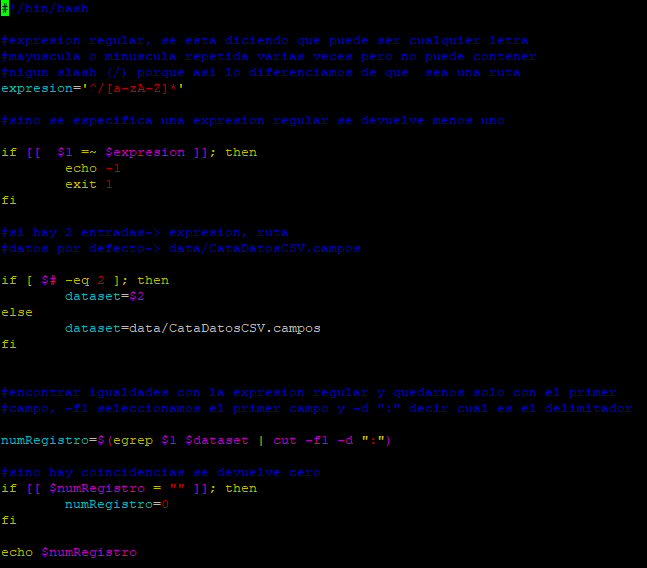
\includegraphics[width=0.60 \textwidth]{Captura.PNG}}
  \caption{Código de fichero \textit{campos2num}.}
\end{figure}

\noindent En la Figura 1 se puede ver la consecución del ejercicio, además está explicada la expresión regular y el por qué de las distintas sentencias. En caso de que no se aprecie bien el código está bien comentado en el programa \textit{bash campos2num}.  \\

\textbf{\section{Generación de algunos listados.}}

\noindent \\ Por último queremos obtener mediante un programa \textit{awk} llamado \textit{listado} el nombre del conjunto de datos (campo número 1), el cual está seguido de ':' y de la fecha de última modificación del dataset (campos número 14). Posteriormente se quiere imprimir en una línea aparte con dos tabuladores el valor de un campo obtenido por el programa \textit{./campo2num}. Para conseguir esto se utilizará la opción \textit{-v}.

\begin{lstlisting}

    #!/user/bin/awk -f
    
    BEGIN{
    
        FS=";";  
    }
    
    #saltar la primera linea
    NR==1{next;}
    
    # ereg es la expresion regular que condiciona el campo x
    # x se obtiene mediante ./campos2num
    $x ~ $ereg{
    
        print $1 ": (" $14 ")\n";
        
        #siendo x el argumento pasado por -v
        print "\t\t" $x; 
    }
    
\end{lstlisting}

\noindent\\ Para ejecutar este programa desde el script \textit{guion} añadimos las siguientes sentencias:
\begin{lstlisting}
    
    #el siguiente codigo es para obtener el mismo resultado que la Figura 3 
    nURL=$(./campos2num 'Enlace al.*')
    
    #el programa convfecha sirve para modificar el formato de las fechas
    awk -f listado -v x=$nURL ereg='.datosabiertos.*' data/CataDatosCSV.csv | 
    sed -f convfecha > data/Figura3
    
\end{lstlisting}

\noindent \\ Por último solo queda mostrar cómo se ha realizado el programa \textit{sed convfecha} para modificar el formato de las fechas. Cabe resaltar que he conseguido obtener la solución esperada pero no de la forma más óptima. Mediante una sola expresión regular solo he conseguido pasar del formato (20180125) al formato [25-01-2018]:

\begin{lstlisting}
    
    # esta expresion regular nos dice que en aquellos sitios donde haya 
    # cuatro numeros (primera condicion) seguidos de otros dos (segunda condicion)
    # seguido de otros dos mas (tercera condicion) los cambiamos a la forma
    # [tercera condicion-segunda condicion-primera condicion] y que reptiamos esto
    # para todas las coincidencias
    
    s/\([0-9]\{4\}\)\([0-9]\{2\}\)\([0-9]\{2\}\)/[\3-\2-\1]/g
    
\end{lstlisting}

\newpage
\noindent \\ El problema lo he encontrado para conseguir obtener [25-ENE-2018] mediante una única expresión regular compacta. Es por esto que he conseguido alcanzar el objetivo pero no de la mejor manera, la solución que he implementado de \textit{convfecha} es la siguiente:

\begin{lstlisting}
    
    #la expresion regular es igual que la explicada anteriormente
    s/\([0-9]\{4\}\)01\([0-9]\{2\}\)/[\2-ENE-\1]/g
    s/\([0-9]\{4\}\)02\([0-9]\{2\}\)/[\2-FEB-\1]/g
    ...
    s/\([0-9]\{4\}\)12\([0-9]\{2\}\)/[\2-DIC-\1]/g
    
\end{lstlisting}

\noindent \\ Utilizando estos programas vamos a crear distintos listados (CataListURLs.list, CataListSectores.list y CataListSectorSalud.list) que almacenaremos en el directorio \textit{data}. Cabe resaltar que para el listado que almacena solo los conjuntos del sector salud he incluido también aquellos sectores mixtos como "medio-ambiente, salud". Añadiremos en el script \textit{guion} lo siguiente:

\begin{lstlisting}
    
    #obtencion del listado de url
    url=$(./campos2num 'Enlace al.*')
    awk -f listado -v x=$url data/CataDatosCSV.csv | sed -f convfecha > 
    data/CataListURLs.list
    
    #obtencion del listado de sectores
    sector=$(./campos2num 'Sector')
    awk -f listado -v x=$sector data/CataDatosCSV.csv | sed -f convfecha > 
    data/CataListSectores.list
    
    #obtencion del listado de sectores de salud
    sector=$(./campos2num 'Sector')
    awk -f listado -v x=$sector ereg='salud' data/CataDatosCSV.csv | 
    sed -f convfecha > data/CataListSectorSalud.list
    
\end{lstlisting}

\noindent \\ Hasta ahora se ha ido indicando qué comandos se han incluido en el script \textit{guion} pero a continuación se va adjuntar un recorte del contenido de forma global para que se vea mejor:

\begin{figure}[H]
  \centering
    \fbox{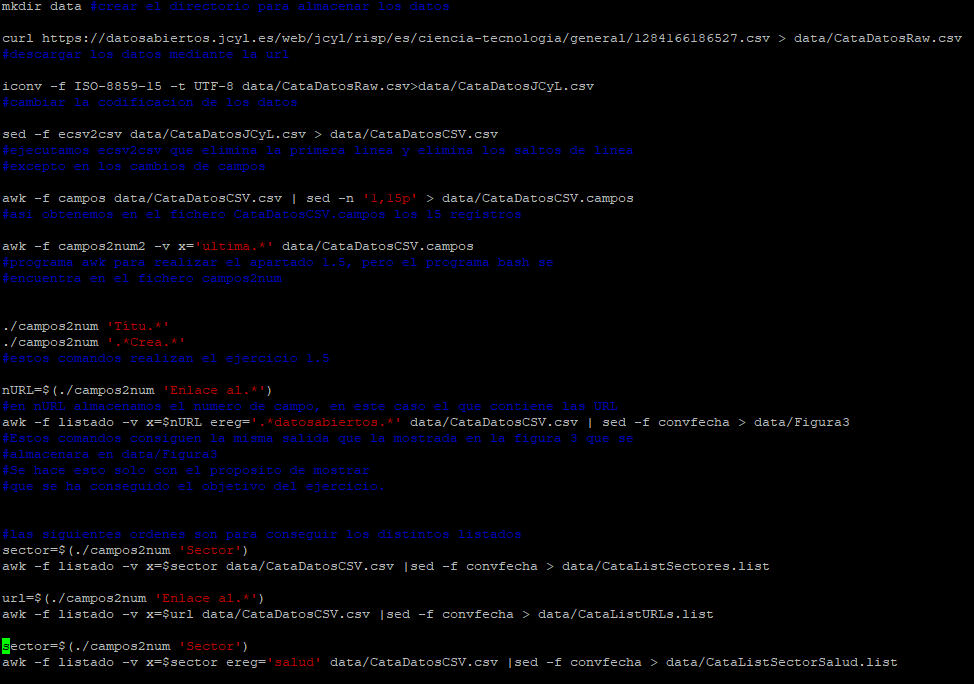
\includegraphics[width=0.75 \textwidth]{Captura2.PNG}}
  \caption{Comandos del script \textit{guion}.}
\end{figure}


\end{document}
